\section{Modellbildung und Regelung}
\label{sec:modelCtrl}
Im ersten Teil \ref{sec:model} dieses Kapitels wird das Fahrzeug modelliert. Dazu wird das Fahrzeug zunächst nach dem Einspurmodell von Ackermann \textbf{QUELLE} modelliert. Anschließend werden die Umsetzung der Stellgrößen des Fahrzeugs in Geschwindigkeit und Lenkwinkel bestimmt. Im zweiten Teil \ref{sec:traj} wird gezeigt, wie aus den erkannten Linien aus Kapitel \ref{sec:linien} eine Trajektorie bestimmt werden kann, welche als Referenzpfad oder zur direkten Steuerung genutzt werden kann. Im letzten Teil werden die zwei getesteten Regelkonzepte erläutert und abschließend eine Beurteilung darüber gegeben.
\subsection{Modellierung}
\subsection*{Ackermann Einspurmodell}\label{sec:model}
Das Fahrzeug wird zunächst mit Hilfe des Einspurmodells nach Ackermann \textbf{QUELLE} modelliert. Das Einspurmodell ist eine übliche Vereinfachung eines vollständigen Modells einen Fahrzeugs mit 4 Rädern. Es fasst jeweils die Vorder- und Hinterräder zu einem in der Längsachse liegendem Rad zusammen. Für das Einspurmodell werden der Radstand und der Schwerpunkt des Fahrzeugs in der Längsachse benötigt. Der Radstand des Fahrzeugs beträgt $L = 0.255 m$. Das Verhältniss zwischen Abstand Hinterachse zum Schwerpunkt zur Hinterachse beträgt ca $0.601$. Mit Hilfe des Einspurmodells kann für einen Lenkwinkel $\delta$ der sich daraus ergebende Kreisradius $R$ bei kontinuierlichem Lenkwinkel berechnet werden.

\begin{figure}[h]
\centering
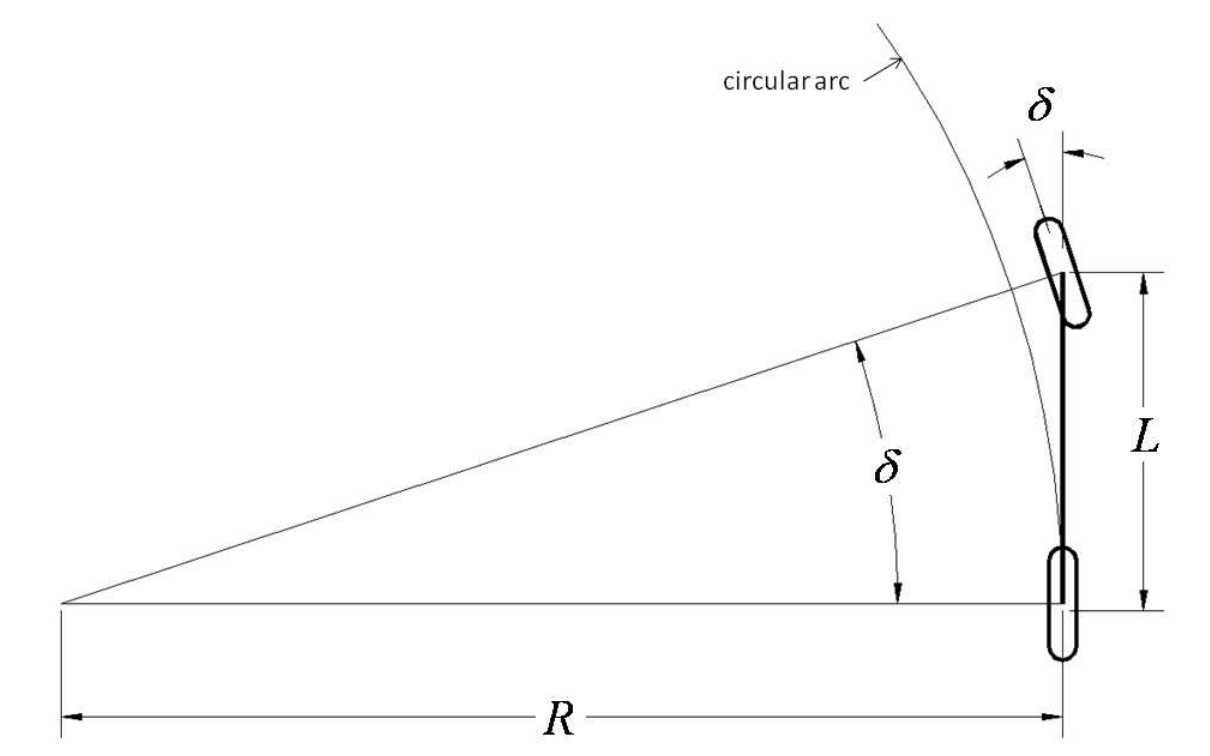
\includegraphics[width = 0.8\textwidth]{../images/ackermann.png}
\caption{Ackermann Einspurmodell \textbf{QUELLE}}
\end{figure}	
	
\subsection*{Bestimmung der Lenkwinkelübersetzung}
Im weiteren wird der Lenkwinkel für verschiedene Stellgrößen bestimmt. Dazu wurde für jeden Lenkwinkel wie folgt vorgegangen.

\begin{itemize}
\item Das Fahrzeug wurde auf seinem Chassi aufgebockt und ein Rad über einem Winkelmesser zentriert.
\item Eine Geschwindigkeit von mindestens 300 (entspricht $~0.5m/s$) wurde eingestellt.
\item Die Lenkvorgabe wurde eingestellt und der Lenkwinkel abgelesen.
\end{itemize}

Aus den sich ergebenden Messpunkten wurde anschließend mit Hilfe von \MATLAB ein sechsten Grades Polynom approximiert:

\begin{align}
\begin{split}
\label{eq:stell(lenkw)}
U(\delta) =&5.726\cdot10^{-6}x^6-35.275\cdot10^{-6}x^5 -0.0044x^4\\ 
&+0.0126x^3+0.6745x^2-43.3355x+59.346
\end{split}
\end{align}

Es ist zu beachten, dass die beiden höchsten Koeffizienten $a_6$ und $a_5$ des Polynoms in Gleichung \ref{eq:stell(lenkw)} sehr klein sind.
	
\begin{figure}[h]
\centering
% This file was created by matlab2tikz.
%
%The latest updates can be retrieved from
%  http://www.mathworks.com/matlabcentral/fileexchange/22022-matlab2tikz-matlab2tikz
%where you can also make suggestions and rate matlab2tikz.
%
%\documentclass[tikz]{standalone}
%\usepackage[T1]{fontenc}
%\usepackage[utf8]{inputenc}
%\usepackage{pgfplots}
%\usepackage{grffile}
%\pgfplotsset{compat=newest}
%\usetikzlibrary{plotmarks}
%\usetikzlibrary{arrows.meta}
%\usepgfplotslibrary{patchplots}
%\usepackage{amsmath}

%\begin{document}
\begin{tikzpicture}

\begin{axis}[%
width=4.521in,
height=3.566in,
at={(0.758in,0.481in)},
scale only axis,
xmin=-25,
xmax=25,
xlabel style={font=\color{white!15!black}},
xlabel={steering Angle in Deg[�]},
ymin=-1000,
ymax=1000,
ylabel style={font=\color{white!15!black}},
ylabel={steering control input},
axis background/.style={fill=white},
axis x line*=bottom,
axis y line*=left,
xmajorgrids,
ymajorgrids,
legend style={legend cell align=left, align=left, draw=white!15!black}
]
\addplot [color=blue, draw=none, mark=*, mark options={solid, blue}, line width=1pt]
  table[row sep=crcr]{%
22	-995.475372508469\\
21	-944.206082620243\\
19	-824.782182082833\\
18	-761.899549732035\\
17	-699.435434651644\\
16	-638.662426049299\\
15	-580.434125640064\\
13	-473.309757857971\\
11	-378.83248310006\\
9.5	-314.975134330865\\
8	-255.370941700404\\
6	-179.364417173131\\
4	-103.534743889814\\
3	-64.6099058087682\\
2	-24.5971862536803\\
1	16.693191571643\\
0	59.3459841555404\\
-1	103.33897644747\\
-2.5	171.536302275685\\
-4	241.606891309475\\
-6	335.761337764135\\
-7.5	404.930495332449\\
-9	471.093087895453\\
-10.5	532.881256459638\\
-13.5	640.760148706949\\
-15.5	703.394004859994\\
-17.5	766.823844751602\\
-20	871.060107107013\\
-20.5	898.97885610975\\
-22	1000.0\\
};
\addlegendentry{measurement}

\addplot [color=green, solid, line width=1pt]
  table[row sep=crcr]{%
22	-995.475372508469\\
21	-944.206082620243\\
19	-824.782182082833\\
17	-699.435434651644\\
16	-638.662426049299\\
15	-580.434125640064\\
13	-473.309757857971\\
11	-378.83248310006\\
9.5	-314.975134330865\\
8	-255.370941700404\\
4	-103.534743889814\\
3	-64.6099058087682\\
2	-24.5971862536803\\
1	16.693191571643\\
0	59.3459841555404\\
-1	103.33897644747\\
-2.5	171.536302275685\\
-4	241.606891309475\\
-6	335.761337764135\\
-7.5	404.930495332449\\
-9	471.093087895453\\
-10.5	532.881256459638\\
-13.5	640.760148706949\\
-15.5	703.394004859994\\
-17.5	766.823844751602\\
-20	871.060107107013\\
-20.5	898.97885610975\\
-22	1006.28525865248\\
};
\addlegendentry{modell}

\end{axis}
\end{tikzpicture}%
%\end{document}

\caption{Lenkwinkel Stellgrößenbestimmung}
\label{fig:lenkgroesse} 
\end{figure}
	
\subsection{Trajektorienberechnung}\label{sec:traj}
\subsection{Regelung}\label{sec:ctrl}